% Format teze zasnovan je na paketu memoir. Prilikom
% zadavanja klase memoir, navedenim opcijama se podešava
% veličina slova (12pt) i jednostrano štampanje (oneside).
\documentclass[12pt,oneside]{memoir}

% Paket koji definiše sve specifičnosti mastera Matematičkog fakulteta.
\usepackage{matfmaster}

% Paket koji obezbeđuje ispravni prikaz ćiriličkih italik slova.
\usepackage{cmsrb}

% Ostali paketi koji se koriste u dokumentu.
\usepackage{listings} % listing programskog koda

% Datoteka sa literaturom u BibTex tj. BibLaTeX/Biber formatu
\bib{hmm_vasovic}

% Ime kandidata na srpskom jeziku (u odabranom pismu)
\autor{Лазар М. Васовић}
% Naslov teze na srpskom jeziku (u odabranom pismu)
\naslov{Скривени Марковљеви модели у биоинформатици}
% Godina u kojoj je teza predana komisiji
\godina{2021}
% Ime i afilijacija mentora (u odabranom pismu)
\mentor{др Јована \textsc{Ковачевић}, доцент\\ Универзитет у Београду, Математички факултет}
% Ime i afilijacija prvog člana komisije (u odabranom pismu)
\komisijaA{... ... \textsc{...}, ...\\ ..., ...}
% Ime i afilijacija drugog člana komisije (u odabranom pismu)
\komisijaB{... ... \textsc{...}, ...\\ ..., ...}
% Datum odbrane (obrisati ili iskomentarisati ako nije poznat)
\datumodbrane{септембар 2021.}

% Apstrakt na srpskom jeziku (u odabranom pismu)
\apstr{%
...
}

% Ključne reči na srpskom jeziku (u odabranom pismu)
\kljucnereci{биоинформатика, скривени Марковљеви модели}

\begin{document}
% ====================================================================
% Uvodni deo teze
\frontmatter
% ====================================================================
% Naslovna strana
\naslovna
% Strana sa podacima o mentoru i članovima komisije
\komisija
% Strana sa podacima o disertaciji na srpskom jeziku
\apstrakt
% Sadržaj teze
\tableofcontents*

% ====================================================================
% Glavni deo teze
\mainmatter
% ====================================================================

% ------------------------------------------------------------------------------
\chapter{Увод}
% ------------------------------------------------------------------------------
Биоинформатика је интердисциплинарна област која се бави применом рачунарских технологија у области биологије и сродних наука, са нагласком на разумевању биолошких података. Кључна особина јој је управо поменута мултидисциплинарност, која се може представити дијаграмом са слике \ref{fig:venn}.

\begin{figure}[!ht]
  \centering
  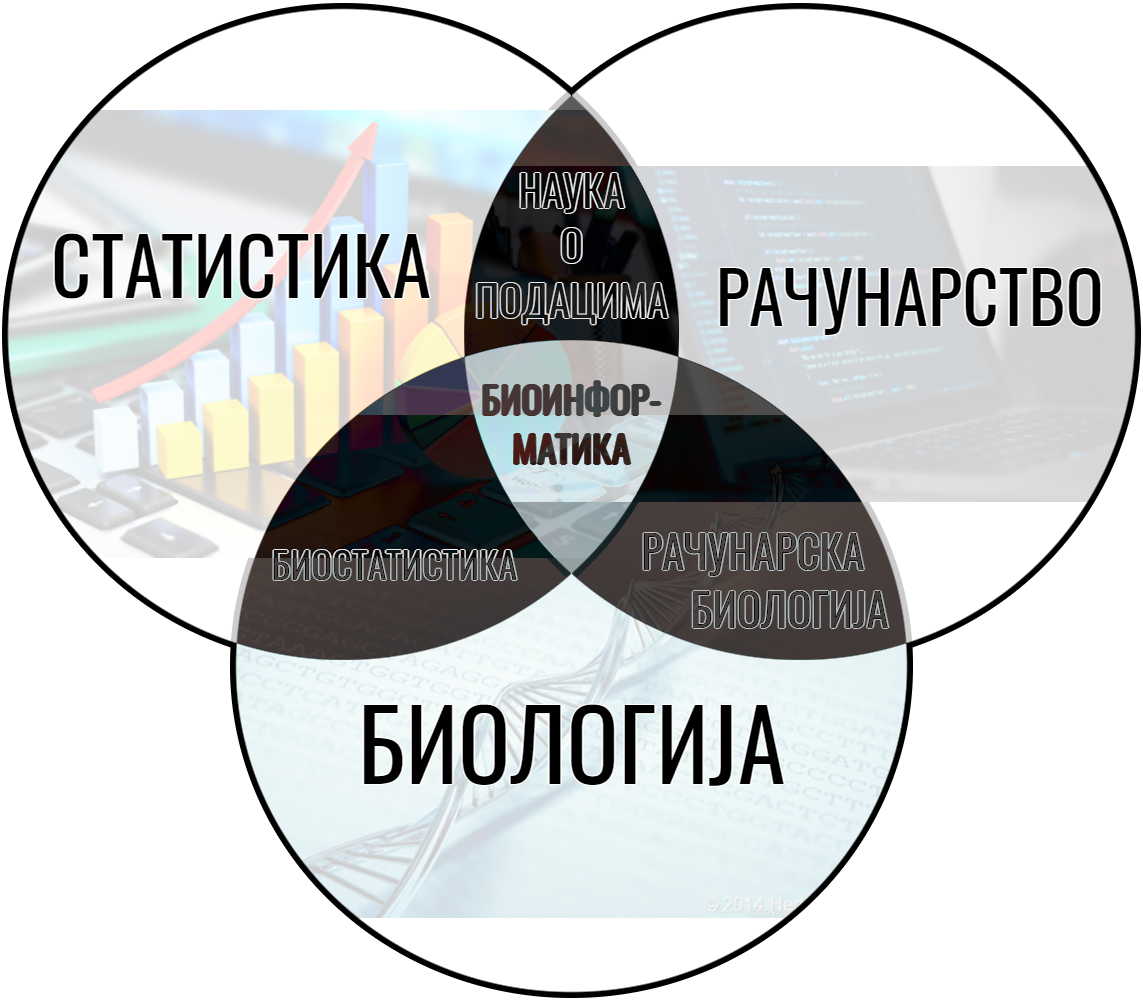
\includegraphics[width=0.75\textwidth]{bioinformatika.png}
  \caption{Венов дијаграм интердисциплинарности\cite{venn}}
  \label{fig:venn}
\end{figure}

Овако представљена, биоинформатика је заправо спој статистике, рачунарства и биологије -- сва три истовремено -- по чему надилази појединачне спојеве: биостатистику, науку о подацима и рачунарску биологију. Конкретно, статистички (математички) апаратат служи за рад са подацима, рачунарске технологије тај апарат чине употребљивијим, док биологија даје потребно доменско знање (разумевање) за рад са биолошким и сродним подацима. Иако се може рећи да је биоинформатика, у савременом смислу представљеном приказаним дијаграмом, релативно млада наука, брзо је постала популарна и многи су јој посветили пажњу или се њоме баве \cite{fauziyyah2019, cmero2015, ufpr}.

Међу познатим личностима из овога домена издвајају се научници Филип Компо (\textit{Phillip Compeau}) и Павел Певзнер (\textit{Pavel Pevzner}), аутори књиге \textit{Bioinformatics Algorithms: An Active Learning Approach}. Прво издање књиге изашло је 2014. године, а друго већ наредне, у два тома. Актуелно, треће издање, издато је 2018. године, у једном тому. Захваљујући динамичном и активном приступу биолошким проблемима и њиховим информатичким решењима, као и многим додатним материјалима за учење, књига се користи као уџбеник на више од сто светских факултета\cite{ba}. Међу њима је и Математички факултет Универзитета у Београду, односно на њему доступни мастер курс Увод у биоинформатику, а делови књиге користе се и у настави повезаног мастер и докторског курса Истраживање података у биоинформатици\cite{matf}.

Актуелна иницијатива на нивоу курса Увод у биоинформатику јесте израда електронског уџбеника, заснованог на поменутој књизи. Идеја је да заинтересовани студенти као мастер рад обраде по једно поглавље књиге, при чему обрада укључује писање текста на српском језику, али и имплементацију и евентуалну визуелизацију свих или макар већине пратећих алгоритама. Овај рад настао је управо у склопу представљене иницијативе, међу првима.

Уџбеник кроз једанаест глава обрађује разне теме које су занимљиве у оквиру биоинформатике: почетак репликације (алгоритамско загревање), генске мотиве (рандомизовани алгоритми), асемблирање генома (графовски алгоритми), секвенцирање антибиотика/пептида (алгоритми грубе силе), поређење и поравнање геномских секвенци (динамичко програмирање), блокове синтеније (комбинаторни алгоритми), филогенију (еволутивна стабла), груписање гена (кластеровање), проналажење шаблона (префиксна и суфиксна стабла), откривање гена и порекла секвенце (скривени Марковљеви модели), напредно секвенцирање пептида (рачунарска протеомика). Циљ овог рада је обрада десетог поглавља, заснованог на скривеним Марковљевим моделима\cite{compeau2015}.

Скривени Марковљев модел (у наставку углавном скраћено \textit{HMM}, према енгл. \textit{Hidden Markov Model}), укратко, представља статистички модел који се састоји из следећих елемената: скривених стања ($x_i$), опсервација ($y_i$), вероватноћа прелаза ($a_{ij}$), полазних ($\pi_i$) и излазних вероватноћа ($b_{ij}$), по примеру са слике \ref{fig:hmm}. \textit{HMM} се тако може схватити као коначни аутомат, при чему стања задржавају уобичајено значење, док вероватноће прелаза описују колико се често неки прелаз реализује. Полазне вероватноће одређују почетно стање. Овакав аутомат допуњује се идејом да свако стање са одређеном излазном вероватноћом емитује (приказује) неку опсервацију. Штавише, најчешће су само опсервације и познате у раду са \textit{HMM}, док се позадински низ стања погађа ("предвиђа"), па се управо зато стања и модели називају скривеним\cite{stamp2021}.

\begin{figure}[!ht]
  \centering
  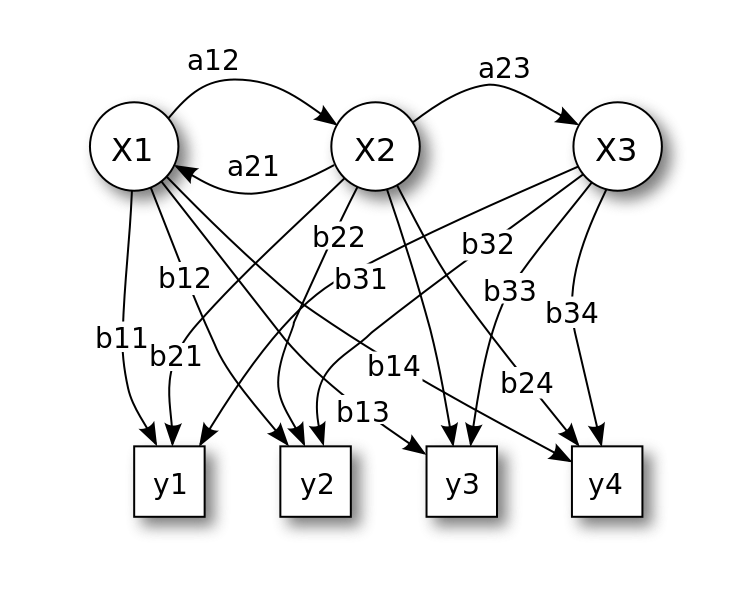
\includegraphics[width=0.75\textwidth]{hmm.png}
  \caption{Једноставан пример скривеног Марковљевог модела\cite{hmm}}
  \label{fig:hmm}
\end{figure}

У претходном пасусу су, наравно, скривени Марковљеви модели представљени малтене само концептуално, на високом нивоу. У наставку ће, међутим, они бити постепено уведени, заједно са мотивацијом за њихову употребу у виду биолошких проблема који се њима решавају. Према идеји електронског уџбеника, излагање ће пратити књигу \textit{Bioinformatics Algorithms: An Active Learning Approach}, а биће имплементирани и сви пратећи алгоритми.

% ------------------------------------------------------------------------------
\chapter{Разрада}
% ------------------------------------------------------------------------------
...

% ------------------------------------------------------------------------------
\chapter{Закључак}
% ------------------------------------------------------------------------------
...

% ------------------------------------------------------------------------------
% Literatura
% ------------------------------------------------------------------------------
\literatura

\end{document}